\section{Grundlagen}
\subsection{Artikel von Maalej und Robillard}
Walid Maalej and Martin P. Robillard ver�ffentlichten  im Septemer 2013 den Artikel "`Patterns of Knowledge in API Reference Documentation"' \cite{MaalejRobillard} und besprechen darin zum Einen eine Taxonomie von in Dokumentationen vorkommenden Wissenstypen und zum Anderen die durchgef�hrte Analyse der Programmiersprachendokumentationen von Java SDK 6 and .NET 4.0. Zum Finden dieser Taxonomie stellten Sie zu jedem neu gefundenen Wissenstyp eine neue Frage auf und erhielten so �ber 100 verschiedene Fragestellungen. Daraufhin wurden �hnliche Fragen zusammengefasst und schlie�lich die 12 in Abbildung~\ref{fig:Wissenstypen_original} gezeigten verschiedenen Wissenstypen ausfindig gemacht.  Auf der Website zu dieser Studie wurde dann zu dem der "`Coding Guide"' \cite{codingguide_orig} ver�ffentlicht, welcher f�r jeden Typ einen Fragenkatalog, Anmerkungen und Beispiele angibt. 
\begin{figure}[h!] 
\centering
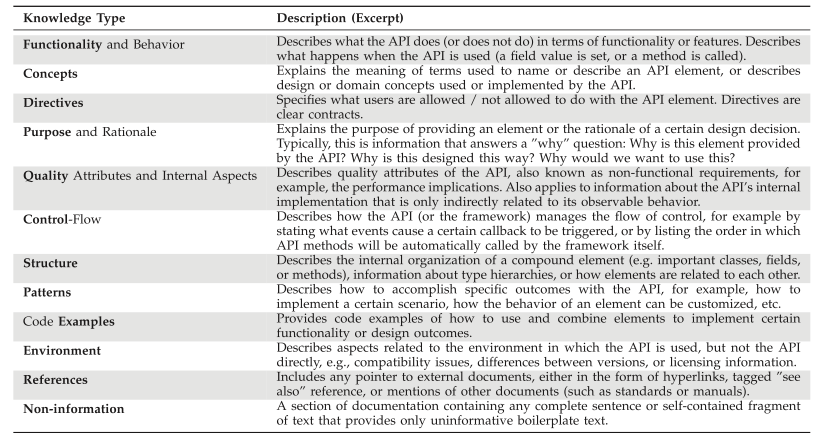
\includegraphics[width=1.1\textwidth]{pictures/knowledgetypes_original.png}
\caption[Wissenstypen in \cite{MaalejRobillard}]{Wissenstypen in \cite{MaalejRobillard}}
\label{fig:Wissenstypen_original}
\end{figure}
Die Vorgehensweise sah vor, dass die Gutachter f�r jeden Wissenstyp bestimmen, ob dieser in der vorgelegten Einheit vorkommt oder nicht. Hierzu konnten f�r jede Einheit die verschiedenen Wissenstypen mit Hilfe von "`CheckBoxes"' angekreuzt werden. 
Jede Einheit wurde von 2 Gutachtern unabh�ngig bewertet. Die Einheiten wurden in drei verschiedene Kategorieren aufgeteilt: 
\begin{enumerate}
\item Module [engl. modules] (entsprechen "`packages"' in Java und "`assemblies"' in .NET)
\item Typen [engl. types] (vor allem Klassen und Schnittstellen)
\item Mitglieder [engl. members] (Felder und Methoden)
\end{enumerate}
Die Einheiten der Kategorie "`Module"' wurden auf Grund der geringen Anzahl, der Unterschiedlichkeit (vor allem bzgl. der L�nge) in Java und .NET und des geringen Informatinosgehalts bei .NET dann aber nicht analysiert. Damit beschr�nkt sich die Original-Studie also auf Typen und Mitglieder. Die Stichprobe �ber die verbleibenden vier Kategorien (zwei je Programmiersprache) wurden mit 95\% Konfidenzintervall und 2,5\% Fehlerspanne gezogen, so dass insgesammt 5.575 Einheiten (431.136 W�rter) zuf�llig ausgew�hlt und auf 17 Gutachter verteilt wurden. \\
So sind insgesamt $5.574 * 2 = 11,148  $ Bewertungen vorgenommen worden. Diese wurden dann im Hinblick auf die �bereinstimmung unter den Gutachtern und bez�glich der Wissenstypen analysiert. Ebenso wurden Auswertungen �ber die F�lle getroffen, in denen sich zwei Gutachter uneinig waren. Zudem konnten so Aussagen dar�ber getroffen werden, welche Wissenstypen bei welcher Einheitskategorie wie h�ufig vorkommen und ob bestimmte Wissenstypen mit einander korrelieren, also  ob z.B. der Typ "'Structure"' h�ufig zusammen mit "`Functionality and Behaviour"' auftritt. Ebenso wurde analysiert, ob und wie ein Zusammenhang zwischen der Anzahl der gefundenen Wissenstypen und der L�nge der Einheiten besteht. \\
Besonders die vorgestellten Wissenstypen und das Kodier-Handbuch [Coding Guide] waren f�r diese Folgestudie sehr n�tzlich und wurden deswegen �bernommen und angepasst. 

\subsection{Kodier-Handbuch}
Das in der Original-Studie \cite{MaalejRobillard} verwendete Kodier-Handbuch findet auch in dieser Studie Verwendung, um von allen Gutachtern die selben bzw. sehr �hnliche Ergebnisse erwarten zu k�nnen. Es dient als Anleitung bei der Bewertung der Einheiten. W�hrend der Gro�teil des Handbuchs �bernommen wurde und unver�ndert bliebt, gab es jedoch ein paar wesentliche Anpassungen. 

\subsubsection{Markierungen}
\label{sec:Markierungen}
Der wichtigste Unterschied zu dem originalen Kodier-Handbuch \cite{codingguide_orig} ist, dass die Gutachtern nicht nur pro Einheit bewerten sollen, ob bestimmte Wissenstypen vorhanden sind, sondern Markierungen in einer Einheit vornehmen und pro Markierung einen Typ festlegen. Wie mit einem Textmarker soll jede Einheit vollst�ndig bearbeitet werden und abschlie�end jedes Zeichen (mit wenigen Ausnahmen) markiert sein. Dies f�hrt zu erg�nzenten Regeln �ber :
\begin{itemize}
\item Die Art Markierungen vorzunehmen
\item Der L�nge von Markierungen
\item Die Notwendigkeit von Doppelmarkierungen in einem Segment
\end{itemize}
Diese �nderungen wurden im ersten Absatz des Kodier-Handbuchs \cite{codingguide_new} wie folgt formuliert: 
\begin{shaded}
You will be presented with documentation blocks extracted from API reference documentation (Javadocs and the like). For each block, you will be also presented with the name of its corresponding package/namespace, class, method, or field. Your task is to read each block carefully and evaluate where the block contains knowledge of the different types described below. Apply the following rules when doing so:
\begin{itemize}
\item Consider the documentation initially one paragraph at a time. If the paragraph contains only information of one knowledge type, mark the whole paragraph with that type in one stretch.
Never mark more than one paragraph at once.
\item If multiple knowledge types mix within the paragraph, mark a contiguous stretch of one or more sentences with one type and the next stretch with another.
\item If necessary, treat subsentences connected with conjunctions such as "`and"', "`or"', "`but"', or with colon or semicolon like complete sentences.
\item A sentence (or such subsentence) as a whole is never marked with more than one type, but sometimes phrases within the sentence will require a separate marking with a different type. Double-marking the same text with two types is allowed (and required) in this case. To create such annotations uniformly, we work in two passes:
\begin{itemize}
\item Pass 1: Prefer longer segments of a complete sentence or several. Annotate subsentences only rarely.
If a sentence contains knowledge of more than one type (which happens quite often), look if one of them is clearly dominant for the overall role of the sentence in the documentation block. If so, annotate only that dominant type to the whole sentence and do not annotate any of the other types yet.
\item Pass 2: After pass 1, many relevant annotations will be missing. We now add those on top of the pass 1 annotations as double annotations. For the double annotations, we still prefer complete subsentences where possible (or other clearly delineated parts such as parentheses), but choose the shorter of two possibilities whenever we are unsure.
\end{itemize}
\item Rate the knowledge type as true only if there is clear evidence that knowledge of that type is present in the stretch.
If you have doubts, consult the type's definition below.
If the doubts do not disappear, do not annotate that type.
\item However, all text of the documentation must be marked with a type. (Only handwritten documentation, not the signature itself and not the placeholders [Something removed here] that indicate left-out nested documentation blocks).
\end{itemize}
Read (and re-read whenever needed) the following descriptions very carefully. They explain how to recognize each knowledge type.
\end{shaded}

\subsubsection{Kleinere �nderungen}
Zudem waren einige kleine �nderungen notwendig, die sich entweder aus dem Stil der Python-Dokumentation ergeben oder als sinnvoller bei der Bewertung von Einheiten ergeben haben. Folgende Semantische �nderungen gab es dabei: 

\begin{itemize}
\item Informationen �ber bestimmten Input einer Funktion oder Methode, welcher zu einer "`Exception"' f�hrt (und nur dann), soll als "`Directive"' und nicht als "`Functionality and Behavior"' markiert werden. 
\item Die simple Nennung von g�ltigen Parametertypen wird als nicht als "`Directive"' angesehen, sofern nicht  Schl�sselw�rter wie "`must"' oder "`have to"' etc. verwendet werden.
\item Der Ausdruck "`Changed in version x.y."' soll als "`Environment"' markiert werden. Der darauf anschlie�end Text kann ebenfalls "`Environment"' sein, muss es aber nicht. 
\item Platzhalter der Form "`[Something removed here]"' sollen nicht markiert und bewertet werden, da diese lediglich auf ausgelassene, verschachtelte Einheiten hinweisen (siehe Abschnitt "`Extrahierer"')
\item Der Wissenstyp "`Structure"' wird treffender in "`Structure and Relationship"' umbenannt. 
\end{itemize}



